\section{Occurrence-event invariants and prime-sensitive obstructions}\label{sec:events}
\subsection{The occurrence fibre}
For an integer state $x$ let $D(x)=\{d\ge2:\ d^2\mid x\}$ be its \emph{occurrence fibre}. A history $h=(x_0,x_1,\dots,x_l)$ induces the \emph{fibre sequence} $D(x_0),\dots,D(x_l)$, and for each index $d\ge2$ the incidence sequence $\rho_d(h)=([d\in D(x_i)])_{i}\in\{0,1\}^{l+1}$.
\begin{lemma}[orthant form]\label{lem:orthant}
$d\in D(x)$ iff $v_p(x)\ge2v_p(d)$ for every prime $p\mid d$. Hence $D(x)=D(x')$ iff $\lfloor v_p(x)/2\rfloor=\lfloor v_p(x')/2\rfloor$ for all $p$, and $\rho_d$ is the indicator of the valuation walk lying in the shifted orthant $O_d=\{v:v_p\ge2v_p(d)\ \forall p\mid d\}$; for a prime power $p^k$ it is the half-space $v_p\ge2k$.
\end{lemma}
\prov{CW-0356}{OCCURRENCE\_BRIDGE:Orthant-form}{PROVED}{FULL}
\begin{lemma}[labels are visible]\label{lem:L}
If $A\ne B$ are both admissible at $x$ then $D(T_Ax)\ne D(T_Bx)$. More precisely some prime $p$ has $|v_p(T_Ax)-v_p(T_Bx)|\ge2$, so $p^k$ lies in exactly one of the two fibres for suitable $k$.
\end{lemma}
\begin{proof}
Since $A+1\ne B+1$ some prime $p$ has, say, $v_p(A+1)>v_p(B+1)\ge0$. Then $p\nmid A$ and $\Delta_p(A)=2v_p(A+1)\ge2$. If $v_p(B+1)\ge1$ then $\Delta_p(B)=2v_p(B+1)$ and the difference is $\ge2$. If $v_p(B+1)=0$ then $\Delta_p(B)=-v_p(B)\le0$ and the difference is $\ge2v_p(A+1)\ge2$. A difference $\ge2$ in $v_p$ gives different integer parts of $v_p/2$.
\end{proof}
\begin{theorem}[faithfulness, locality, event locality]\label{thm:faith}
(a) For a fixed source the fibre sequence $F(h)$ determines the history $h$. (b) A legal swap changes exactly one entry of $F(h)$; hence the occurrence signature is never a swap invariant, and swaps preserve exactly the source, content, endpoint and all but one fibre. (c) If $d$ is lost at a step with label $N$ then $\gcd(d,N)>1$; if $d$ is born then $\gcd(d,N+1)>1$; the label $1$ never causes a loss.
\end{theorem}
\begin{proof}
(a) Induction on length: given $x_{j-1}$, \cref{lem:L} says the fibre $D(x_j)$ determines $N_j$ among the labels admissible at $x_{j-1}$. (b) A swap at position $i$ changes only the intermediate state; the two intermediate states are $T_Ax$ and $T_Bx$ with different fibres by \cref{lem:L}. (c) If $d\in D(x)\setminus D(Tx)$ there is $p\mid d$ with $v_p$ falling below $2v_p(d)$, so $\Delta_p(N)<0$, i.e.\ $p\mid N$. If $d$ is born then $\Delta_p(N)>0$ for some $p\mid d$, so $p\mid N+1$. Finally $\Delta_p(1)=2v_p(2)\ge0$.
\end{proof}
\prov{CW-0341}{D-T4}{PROVED}{FULL}
\emph{Corollary.} Histories with the same source and endpoint have pairwise different fibre sequences even when they are swap-equivalent: the endpoint keeps only the last entry. In the benchmark of $72$, $\rho_2(h_1)=(0,1,1,1)$ and $\rho_2(h_2)=(0,1,0,1)$ for the two swap-equivalent histories. Finite-exact check: $0$ collisions among $104$ histories and among $13\,950$ label pairs.
\begin{proposition}[local discrepancy]\label{prop:discrepancy}
For a legal swap with intermediate states $a=T_Ax$, $b=T_Bx$ and half-valuation vectors $e_p=\lfloor v_p/2\rfloor$, the changed entry differs by
\[|D(a)\,\triangle\,D(b)|=\prod_p(e_p(a)+1)+\prod_p(e_p(b)+1)-2\prod_p(\min(e_p(a),e_p(b))+1)>0,\]
because $D(a)\cap D(b)=D(\min(e(a),e(b)))$ and $|D(x)|=\prod_p(e_p(x)+1)-1$. The swap preserves $\rho_d$ iff $d\notin D(a)\triangle D(b)$, i.e.\ iff $a$ and $b$ lie on the same side of the orthant $O_d$.
\end{proposition}
\prov{CW-0357}{OCCURRENCE\_BRIDGE:Local-discrepancy}{PROVED}{FULL}

\subsection{Persistence-restricted swap connectivity}
For an index $d\ge2$ keep a legal swap in the \emph{preserve} mode iff $d\notin D(a)\triangle D(b)$; in the \emph{after-birth} mode iff that holds or $d$ occurs in none of $D(x_0),\dots,D(x_i)$. Both modes delete edges, so
\[\#\text{classes(unrestricted)}\le\#\text{classes(after birth)}\le\#\text{classes(preserve)}\]
(proved: deleting edges cannot decrease the component count; the after-birth edge set contains the preserve edge set). Restricting by all indices at once leaves no edge (\cref{lem:L}); a single index $d$ is the reduced, informative property.
\begin{table}[tbp]\centering\small
\begin{tabular}{@{}rrrrrrrrrr@{}}\toprule
$r$ & hist. & classes & pres.\ 2 & pres.\ 3 & pres.\ 4 & pres.\ 8 & aft.\ 2 & aft.\ 3 & pres.\ 12 / 36\\\midrule
1 & 4 & 3 & 4 & 4 & 4 & 3 & 4 & 3 & 3 / 3\\
2 & 100 & 22 & 36 & 51 & 62 & 54 & 32 & 24 & 43 / 33\\
3 & 3\,601 & 142 & 413 & 551 & 864 & 1\,009 & 355 & 239 & 678 / 493\\\bottomrule
\end{tabular}
\caption{\textbf{Swap classes of the complete histories of $72^r$ under persistence restriction (finite-exact; recomputed in this work).} ``pres.\ $d$'' and ``aft.\ $d$'' are the numbers of classes in the preserve and after-birth modes for the index $d$. The unrestricted counts are $3,22,142$.}\label{tab:persist}
\end{table}
\begin{proposition}[finite-exact: persistence restriction is strictly finer and not monotone in $d$]\label{prop:persist}
(1) Restricted connectivity is strictly finer than unrestricted already at $r=1$: for $d=2$ the histories $h_1,h_2$ of $72$ (swap-equivalent) are separated, $4$ classes instead of $3$. (2) The number of classes is not monotone along divisibility of $d$: for $r=3$ the index $d=12$ gives $678$ classes and $d=36$ gives $493$, though $12\mid36$ (for $r=2$: $43$ and $33$). (3) After-birth is coarser than preserve. \stat{finite-exact} for $r\le3$; no counting law in $r$ is known.
\end{proposition}
\prov{CW-0358}{OCCURRENCE\_BRIDGE:Results}{FINITE-EXACT}{FINITE}

\subsection{Churn}
For a history of length $l$ put $V_d=\sum_i|\rho_d(i+1)-\rho_d(i)|$ and $\chi_d=\tfrac12\bigl(V_d-|\rho_d(l)-\rho_d(0)|\bigr)$, the \emph{reduced churn} (the number of lost-and-regained or gained-and-lost excursions).
\begin{theorem}[churn bounds]\label{thm:churn}
(i) $\chi_d\le\lfloor l/2\rfloor$. (ii) A swap changes one entry of $\rho_d$, so $|\chi_d(h)-\chi_d(h')|\le1$ for swap-adjacent $h,h'$. (iii) If $\Delta_p(N)\ge0$ for all labels $N$ of $h$ and primes $p\mid d$, then $\rho_d$ is nondecreasing and $\chi_d=0$ (for instance $h_{\mathrm A}=1^7$). (iv) \emph{Dip lemma:} if $v_p$ dips to at least $2$ below its start value $a$ and ends at or above $a$, then $\chi_{p^{\lfloor a/2\rfloor}}\ge1$.
\end{theorem}
\begin{proof}
(i) $V_d\le l$ and $V_d\equiv|\rho_d(l)-\rho_d(0)|\pmod 2$, so $2\chi_d\le l$. (ii) Changing one interior entry of a $0/1$ sequence changes $V_d$ by at most $2$ and leaves the end values alone. (iii) $v_p$ is then nondecreasing for $p\mid d$, so $\rho_d$ is. (iv) With $k=\lfloor a/2\rfloor$: the start has $v_p=a\ge 2k$, so $\rho=1$; at the dip $v_p\le a-2<2k$ (as $2k\ge a-1$), so $\rho=0$; the end has $v_p\ge a\ge 2k$, so $\rho=1$; hence $V\ge2$ and $\chi\ge1$.
\end{proof}
\prov{CW-0389}{B-T7}{PROVED}{FULL}
\begin{theorem}[necessary churn of the merger]\label{thm:churnmerger}
For every source $m$ and every admissible arrangement of $\{2^2,3^4\}$ some $d$ has $\chi_d\ge1$, whereas $\chi_d(1^7)=0$ for all $d$. Hence every endpoint-preserving rewrite between $1^7$ and an arrangement of $\{2^2,3^4\}$ creates an occurrence gap.
\end{theorem}
\begin{proof}
The walk $v_3$ starts at $b=v_3(m)$ and has steps $+2$ (twice, labels $2$) and $-1$ (four times, labels $3$), ending at $b$, and stays $\ge0$. Take $d=3^k$, so $\rho_d=[v_3\ge2k]$.
\emph{Case 1:} the walk reaches $b+2$. Put $k=\lfloor b/2\rfloor+1\ge1$; then $2k\ge b+1>b$ and $2k\le b+2$, so $\rho=0$ at the start and the end, and $\rho=1$ at the moment of reaching $b+2$: $\chi\ge1$.
\emph{Case 2:} the walk stays $\le b+1$. Its first step cannot be $+2$, so it is $-1$ and the walk reaches $b-1$ (so $b\ge1$). If $b$ is even put $k=b/2\ge1$: $\rho=1$ at start and end ($v_3=b=2k$) and $\rho=0$ at $b-1$. If $b$ is odd and the walk reaches $b-2$ or lower put $k=(b-1)/2$: start and end have $\rho=1$ ($b\ge2k$), the low point has $v_3\le b-2<2k$. If $b$ is odd and the walk never goes below $b-1$, it can leave $b-1$ only by a $+2$ step, so it visits $b+1$; with $k=(b+1)/2$, $\rho=0$ at the start and end and $\rho=1$ at $b+1$. In each case $V_d\ge2$ and $\chi_d\ge1$. For $1^7$ every $\Delta_p(1)\ge0$, so \cref{thm:churn}(iii) gives $\chi_d=0$.
\end{proof}
\prov{CW-0390}{B-T8}{PROVED}{FULL}
\emph{Check.} All arrangements for $v_2(m)\le8$, $v_3(m)\le6$ ($690$ admissible cases) and the monotone and dip statements ($1126$ and $2162$ cases) were replayed with no violation. In the block cube family from $4$ the total churn at source $4$ equals the number of $\mathrm B$-blocks; the minimum number of churning indices over all sources and arrangements within the tested index set is $5$ (cited).

\subsection{Information across rewrites}
\begin{proposition}[births minus losses is a rewrite invariant]\label{prop:births}
Let $\mathrm{births}$ and $\mathrm{losses}$ be the numbers of index-birth and index-loss events along a history. Then $\mathrm{births}-\mathrm{losses}=|D(x_l)|-|D(x_0)|$ depends only on the endpoint and the source, so it is a rewrite invariant. The fibre sequences are \emph{not} rewrite invariants (rewrites change lengths). In the cube family of \cref{thm:cubefam}, $\mathrm A$ has $(\mathrm{births},\mathrm{losses})=(7,0)$ and $\mathrm B$ has $(14,7)$, with difference $7$ each; the $2^r$ histories of the cube family are pairwise distinguished by their fibre sequences for $r\le4$, while the pairs $(\mathrm{births},\mathrm{losses})$ take $2,4,8,15,24$ distinct values for $r=1,\dots,5$, so that the pair is a faithful label only for $r\le3$. The first statement is proved by telescoping; the numerical statements are \stat{finite-exact} and cited.
\end{proposition}
\prov{CW-0382}{D4-T9}{PROVED}{FULL}
The endpoint fixes the image $V_Ac$ and leaves the position in the kernel coset free; block rewrites move within that coset, and a telescoping invariant such as $\mathrm{births}-\mathrm{losses}$ depends on the endpoint alone and so cannot see that position.

\subsection{A separator of swap classes by one occurrence index}
\begin{theorem}[the order of $2$ and $4$; proved-scoped]\label{thm:R3T3}
Let $A$ be a set of distinct labels with $A\cap\{1,2,4\}=\emptyset$, let the source be $4$ and the content $C=\{2,4\}\cup A$. For an admissible arrangement $w$ of $C$ put $I(w)=1$ if $2$ precedes $4$ and $I(w)=0$ otherwise. Then $I$ is constant on swap classes. Consequently the number of swap classes is at least the number of values of $I$ that occur.
\end{theorem}
\begin{proof}
A swap exchanging two labels other than the pair $\{2,4\}$ does not change the relative order of $2$ and $4$. A legal swap of $2$ and $4$ requires them to be adjacent with $8=2\cdot4$ dividing the state $x$ before the pair (\cref{prop:diamond}). If the pair is not at the first two positions, the first label of the history lies in $A$; but at the source $4$ the only applicable labels are the divisors $1,2,4$ of $4$, and $A$ contains none of them. So the pair occupies the first two positions and $x=4$, and $8\nmid4$.
\end{proof}
\provx{R3-T3}{CW-0413/0414 (proposed co-located proof)}{proved-scoped}{full}
\begin{example}[the family from endpoint $9000$]\label{ex:R3T3}
For $A=\{5,9\}$ the content $\{2,4,5,9\}$ ends at $9000$ and has $2$ swap classes, each of $2$ histories: $\{(2,9,4,5),(2,9,5,4)\}$ with $I=1$ and $\{(4,5,2,9),(4,5,9,2)\}$ with $I=0$ (\cref{fig:occur}). For $A=\{3,5,9\}$ (endpoint $48000$) there are $3$ classes (sizes $1,3,4$) with $I$-values $1,1,0$, and for $A=\{3,5,6,9\}$ (endpoint $392000$) there are $3$ classes (sizes $5,8,14$) with the same $I$-values: $I$ separates the pair of values but is not a complete invariant. In a sweep over all $39$ subsets $A\subseteq\{3,\dots,12\}$ of size $1$ to $3$ the invariance of $I$ holds in all cases ($0$ violations); the number of classes is $1$ for $24$ contents, $2$ for $14$ and $3$ for $1$, and both values of $I$ occur for $14$. \stat{finite-exact}. The classification of the classes beyond $I$ is not given.
\end{example}
\begin{figure}[tbp]\centering
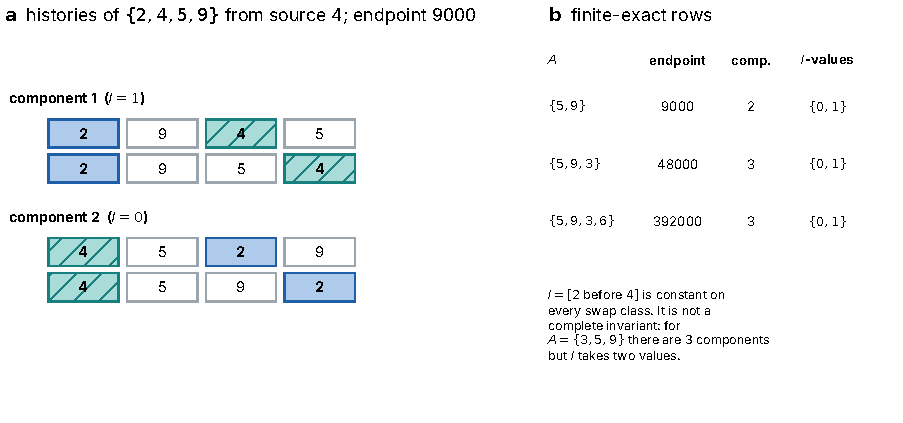
\includegraphics[width=\linewidth]{fig19_occurrence_events}
\caption{\textbf{The order of $2$ and $4$ separates swap classes (finite-exact data, theorem exact).} (a) The four histories of the content $\{2,4,5,9\}$ from source $4$ (endpoint $9000$) grouped into the two swap classes; the labels $2$ (light fill) and $4$ (hatched) are marked, with $I=[2$ before $4]$. (b) The three rows computed: the sets $A$, endpoints, number of components and values of $I$; for $A=\{3,5,9\}$ there are $3$ components but $I$ takes two values only. Theorem illustrated: \cref{thm:R3T3}.}\label{fig:occur}
\end{figure}
\begin{remark}[a corrected statement]\label{rem:B2T9}
The square-root content $\sigma(x)=\prod_pp^{\lfloor v_p(x)/2\rfloor}$ has $D(x)$ as its set of divisors $\ge2$, and along every SELECT-II edge $\sigma'/\sigma=(N+1)/c>1$ with $c\le N$ the product of the prime powers $p^{\lfloor\cdot/2\rfloor}$ or $p^{\lceil\cdot/2\rceil}$ taken from $N$ (the programme's B2-T9, ``no silent step''). The inclusion $D(x)\subsetneq D(x')$ that was once stated with it does \emph{not} hold, as the accepted erratum records: $4\to18$ has $D(4)=\{2\}$ and $D(18)=\{3\}$. The occurrence fibre is therefore not monotone along histories, which is why churn is a meaningful quantity. \stat{cited}.
\end{remark}
